\documentclass[11pt,onecolumn]{article} 

\usepackage{latex8}
\bibliographystyle{latex8}

\usepackage{times}

% for highlighting todos and fixes
\usepackage{color, soul}

% for figures
\usepackage{caption}
\usepackage{graphicx}

\usepackage{amsmath}
\usepackage{setspace}

% for references and urls
\usepackage{url}
%\usepackage{hyperref} % we can use this, but it makes a weird table of contents with the formatting we are using

\newcommand{\h}[1]{\hl{#1}}

\singlespacing	% we can bump this to \onehalfspacing to increase readability if you want

\begin{document}

\title{Clever Title}

\author{
 Aaron Stacy \\ \and
 Calvin MacKenzie \\
}

\maketitle

\Section{Introduction}

Originally developed by Andrew Viterbi to decode signals over noisy channels, the Viterbi algorithm proved to be useful in a wide variety of areas. Within the field of Natural Language Processing (NLP), the Viterbi algorithm is most commonly used with Hidden Markov Models (HMM) to find the most likely sequence of part-of-speech tags, and other related tagging tasks.

Closely related to the Viterbi algorithm is the Forward algorithm, which is used within NLP to efficiently compute observation likelihood. While not as popular as the Viterbi algorithm, the Forward algorithm is a fundamental algorithm within NLP. The implementations of the two algorithms are actually quite similar and they share the same running time of $O(T N^2)$.

Work on improving the Viterbi algorithm typically comes from the realm of signal processing, rather than NLP, where these gains greatly help with the decoding of signals. Typically, these improvements deal with a hardware viterbi decoder and ways to modify this hardware in order to enhance the parallelization of the decoding problem.

Rather than approaching this task from a hardware perspective, we wanted to improve these algorithms with parallelization techniques. We implemented a parallel version of the Viterbi and Forward algorithms using the OpenMP API \footnote{\url{http://openmp.org/wp/}} and characterized the performance over a range of workloads. We tested this on the Wall Street Journal dataset from the Penn Treebank and varied the size of the dataset to measure performance. We ran the algorithm on the TACC cluster in order to find strong and weak scaling characteristics.

\Section{Related Work}

\begin{figure}[h!]
\centering
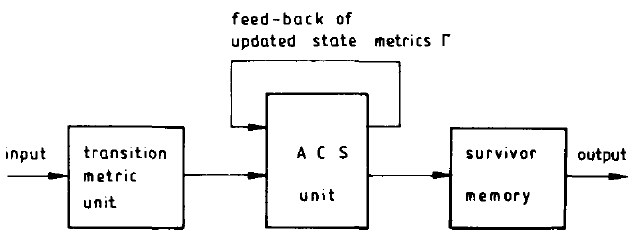
\includegraphics[width=.5\linewidth]{figures/pipeline}
\caption{Pipeline structure of Viterbi decoder}
\label{fig:pipeline}
\end{figure}

The work by Fettweis and Meyr (1989) \cite{acs:old} describes a successful attempt at parallelizing a key bottleneck of the Viterbi algorithm: the add-compare-select component. The authors describe the process of obtaining the updated state metric, $\Gamma_{n+1,z_{i}}$, as the add-compare-select (ACS) unit of the Viterbi algorithm, shown in Figure \ref{fig:pipeline}. The formula to find this updated state is shown below (where $\lambda$ is the transition probability):

\begin{equation}
\Gamma_{n+1,z_{i}} = \max\limits_{\text{all possible } z_{k}\rightarrow z_{i}} (\Gamma_{n,z_{k}} + \lambda_{n,z_{k}\rightarrow z_{i}})
\end{equation}

This equation is at the heart of the Viterbi algorithm, and forces the current state to depend on all previous states with its recursive nature. 

Even though the ACS unit is only one component of the Viterbi algorithm, the authors explain that ``since the ACS unit is much more complex, it is the bottleneck which limits the throughput rate.'' To combat this, the authors introduce the concept of an $M$-step trellis, as opposed to the traditional 1-step trellis used in the Viterbi algorithm. This can be used in the ACS loop, but will take $M$ times as long. Utilizing a combination of the original 1-step trellis and the $M$-step trellis allows the authors to parallelize the Viterbi algorithm in combination with a multiplexer.

\begin{figure}[h!]
\centering
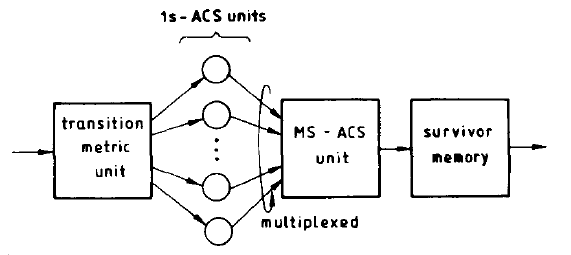
\includegraphics[width=.5\linewidth]{figures/pipeline_multiplex}
\caption{Multiplexed structure of Viterbi decoder}
\label{fig:pipeline_multiplex}
\end{figure}

The new pipeline structure is shown in Figure \ref{fig:pipeline_multiplex}. This is implemented in hardware using a systolic array, which is a pipelined structure of processing units called cells. Each of these cells can be computing in parallel and combined at the end, speeding up the overall process.\\

Du et al. \cite{gatech:bio} proposed extensions to two known methods for parallelizing the computationally intensive kernel of the Viterbi algorithm. The paper is applied to computational biology, so the authors first investigate existing parallelization methods for related sequence alignment algorithms.

The authors also demonstrate how to divide the Viterbi algorithm into two parts: independent sections of the calculation do not depend on previous results, and are therefore more amenable to parallelization. By isolating the dependent ant parts of the computation, the sequential work is minimized and the authors achieve greater speedup.

Because of the difference in application domain, the specifics of the approach taken by Bader et al. cannot be directly applied to NLP. However when designing parallel algorithms the basic principles of locality always apply. There are two specific techniques used by Bader et al. that can be applied to a more general Viterbi algorithm: dividing dependent and independent calculations and streaming algorithms that overlap data transfer with calculation. We were able to use the latter in our implementation.

\Section{Method Overview}

\SubSection{Subsection}

\Section{Experimental Evaluation}

\SubSection{Methodology}

\SubSection{Results}

\Section{Future Work}

\Section{Conclusion}

\begin{thebibliography}{1}
\small

\bibitem{gatech:bio}
Z. Du, Z. Yin, and D. Bader. A tile-based parallel Viterbi algorithm for biological sequence alignment on GPU with CUDA. \emph{Parallel \& Distributed Processing, Workshops and Phd Forum (IPDPSW), 2010 IEEE International Symposium on. IEEE}, 2010.

\bibitem{acs:old}
G. Fettweis, \& H. Meyr. Parallel Viterbi algorithm implementation: Breaking the ACS-bottleneck. \emph{Communications, IEEE Transactions on}, 37(8), 785-790,  1989.

%Author 1, Author 2. Title. \emph{Conference}, Year.

\end{thebibliography}

\end{document}


